\chapter{The LUX and LZ experiments}
Currently the most stringent limits on WIMP mass and cross section are set by the Large Underground Xenon (LUX) detector. The LUX-ZEPLIN (LZ) detector will be the successor to LUX and will have roughly 200 times greater sensitivity than LUX. LUX and LZ are two-phase xenon time-projection chambers (TPC's) designed to detect relic WIMPs in the local galactic halo scattering off of the target xenon nuclei. 

If a WIMP interacts with one of the target atoms, it will deposit energy in the form of freed electrons, light, and heat. Two arrays of photo-multiplier tubes (PMT's) at the top and bottom of the detector detect the light emitted from this interaction as primary scintillation (S1). The electrons are drifted through an electric field to the top of the liquid where they are extracted and cause secondary scintillation light (S2) which is also detected by the PMT's. The x-y position of this event can be reconstructed mapping the relative signals from the S2 in the top PMT array. The depth of the event is given by the time separation between the S1 and S2. The relative size of the S1 and S2 will be different depending on whether the interaction was with the xenon nucleus or an orbital electron. A WIMP will interact coherently with the nucleus, so it is 132 times more likely to interact with a xenon nucleus than with an electron. Since most of the background events in LUX are from gammas and betas, which interact with the orbital electrons, the ratio of S2 to S1 can be used to efficiently discriminate between background and signal.

\begin{figure}[h!]
\centering
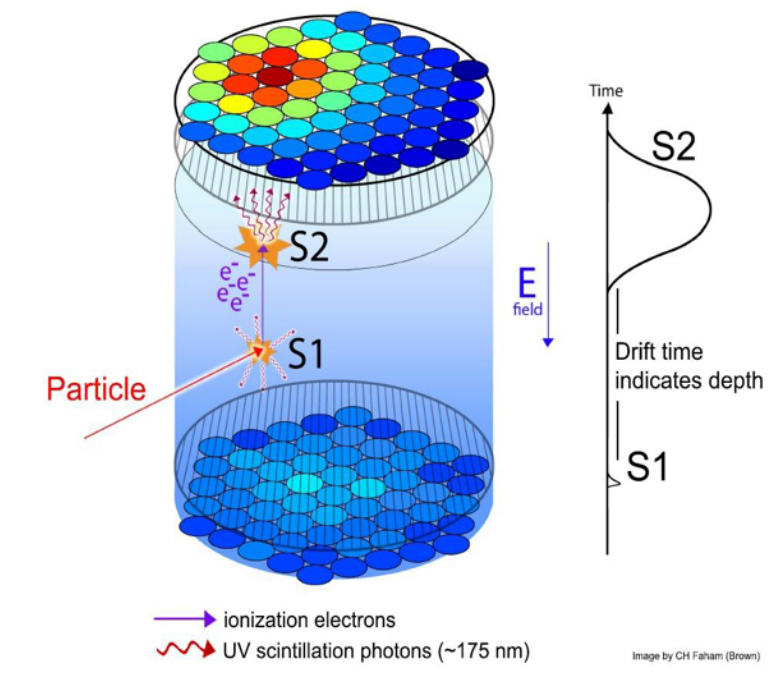
\includegraphics[width=150mm]{Figures/luxevent.png}
\caption{Schematic drawing of and event in the LUX detector.\cite{lux2012}}
\label{fig:lux} 
\end{figure}

 LUX is currently located at the Sanford Underground Research Facility in Lead South Dakota. It is 4850 feet underground (4300 m w.e.). The detector itself is immersed in a large water tank to shield it from neutrons and gammas. LUX contains about 370 kg of xenon, and uses a fiducial volume containing about 118 kg as its WIMP target. The remaining xenon acts as a shield from external gammas and betas. 
 
 \section{The libNEST Model of the LUX Detector}\label{sec:libnest}
 
 \subsection{Detector Resolution for Charge and Light Signals}\label{sec:detres}
 
 The S1 detector resolution, $\sigma_{\gamma,det}$ is composed of three parts; the binomial variance due to the finite light collection efficiency, $\epsilon_{\gamma}$:
\begin{equation}
\sigma_{S1,col}^2=N_{\gamma}G1(1-G1), 
\end{equation}
an additional variance due to a nonzero probability, $P_{DPE}$, that the PMT will experience double-photoemission\cite{DPE}:
\begin{equation}
\sigma_{S1,DPE}^2=G1\cdot N_{\gamma}P_{DPE}(1-P_{DPE}), 
\end{equation}
and the variance due to finite PMT resolution, $\sigma_{PMT}$:
\begin{equation}
\sigma_{S1,PMT}=N_{\gamma}G1\sigma_{PMT}^2
\end{equation}
For LUX we have $G1\approx 0.095$, $P_{DPE}\approx 0.2$, and $\sigma_{PMT}\approx 0.50$. Put together, this gives:
\begin{equation}
\begin{split}
\sigma_{S1}^2&=N_{\gamma}G1(1-G1+P_{DPE}(1-P_{DPE})+\sigma_{PMT}^2)\\
&\approx 0.125 N_{\gamma} \ \ (\text{phd}^2),
\end{split}
\end{equation}
or:
\begin{equation}
\sigma_{\gamma,det}=\sigma_{S1}/G1=3.7 \sqrt{N_{gamma}} \ \  (\text{phd})
\end{equation}
 
 \section{Electric Field Model}\label{sec:efield}
 \cite{lux_efield}
 
 
 \section{Efficiency Corrections}\label{sec:krypcal}
 In run 4, the position-dependent efficiency corrections for the LUX S1 and S2 signals were obtained from a combination of tritium and $^{83m}$Kr calibration data using a procedure referred to as KrypCal\cite{richard}.  
 
\section{Electron Trains in LUX Run04} \label{sec:etrain}
 